\subsection{Blockchain}
\label{sec:sota_blockchain}

    Quellen: \cite{Dorri2016}\cite{Conoscenti2016}\cite{Greenspan2015}\cite{ISO307}\cite{Kshetri2017}\cite{Nakamoto2008}\cite{Underwood2016}\cite{Vukolic2016}\cite{Vukolic2017}\cite{Wuest2017}\cite{Zheng2017}
    
    \subsubsection{Einführung in das Konzept}
    \label{sec:sota_blockchain_introduction}
    Eine Blockchain ist in ihrer Essenz eine immer länger werdende, unveränderbare, öffentliche Kette von Transaktionen, die dezentral gespeichert wird (s. \fref{fig:bc_highlvl}). 
    
    \begin{figure}[H]
    	\centering
    	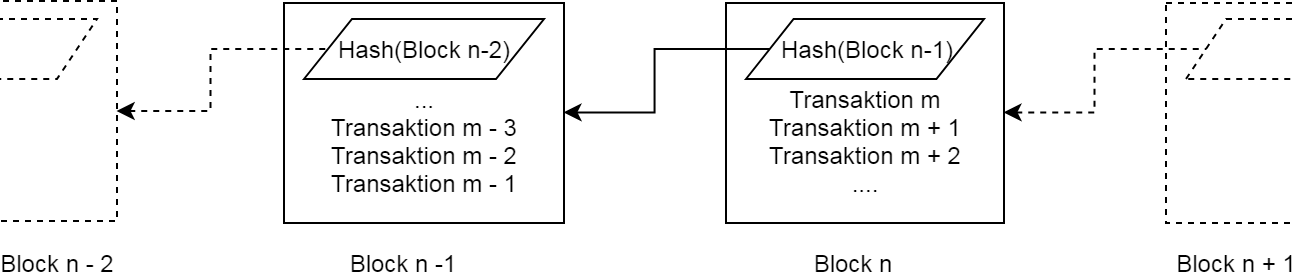
\includegraphics[width=\textwidth]{graphics/bc_highlvl.png}
    	\caption{Abstrakte Darstellung einer Blockchain}
    	\label{fig:bc_highlvl}
    \end{figure}
    \noindent Erstmals 2008 von Satoshi Nakamoto, ursprünglich als Peer-to-Peer Electronic Cash System ,,Bitcoin`` (heute als eine sogenannte Kryptowährung bekannt) erfunden, fand die Technologie aufgrund ihrer Eigenschaften wie ihres dezentralen, anonymen Konzepts schnell viele Sympathisanten. 
    Bitcoin ist die erste populäre digitale Währung, die ohne zentrale Autorität wie beispielsweise einer \gls{ttp} das in \fref{sec:sota_doublespend} vorgestellte Double-Spending Problem lösen sollte\cite{Nakamoto2008}. 
    Übertragen auf Bitcoin bedeutet es, dass ein Empfänger einer Transaktion sichergehen können muss, dass der vorige Besitzer den Bitcoin oder den Bruchteil dessen vorher nicht schon einmal an einen anderen Empfänger gesendet hat.
    Dies wird mittels kryptographischem Beweis, welcher im folgenden Abschnitt genauer betrachtet wird, anstatt des laut \citeauthor{Nakamoto2008} vorstellten mangelhaften Modells der \gls{ttp}, welche stets einen Single Point of Failure
    \!\footnote{Ein Single Point of Failure stellt beipsielsweise eine Bank im Zahlungsverkehr dar.
    Fällt die Bank beispsielsweise aus irgendeinem Grund aus, haben deren Kunden keine Möglichkeit mehr Überweisungen von und zu ihren Konten zu tätigen.}
    darstellt, gelöst. 
    Das Konzept ermöglicht es somit zwei Entitäten, die sich gegenseitig nicht zwingend vertrauen müssen, um eine sichere (im Sinne der Vertraulichkeit) direkte Transaktion miteinander durchzuführen.
    
    \noindent Grundlegend ist die Blockchain eine verteilte Datenstruktur, die zwischen den Mitgliedern eines Netzwerkes repliziert und geteilt wird\cite{Christidis2016}.
    Die Knoten des Netzwerkes (genannt ,,Miner'`) fügen validierte, gegenseitig abgestimmte Transaktionen zwischen Teilnehmern, die zu Blöcken gebündelt werden.
    Die Blockchain beinhaltet das maßgebliche ,,Hauptbuch'` von Transaktionen, welches im Endeffekt festlegt, wem was gehört.\todo[color=yellow]{meh}
    Dieses ,,Hauptbuch'` ist ein Log, dessen Einträge mit Zeitstempeln jeweils als Blöcke zusammengefasst werden.
    Das System ist so lange sicher, wie ,,ehrliche'` Knoten gemeinsam mehr Rechenleistung als eventuell zusammenarbeitende Angreifer haben\cite{Nakamoto2008}.
    
    
    %% Transaktionen
    Getätigte Transaktionen sollen nicht mehr rückgängig gemacht werden können.
    Erreicht wird dies, indem die Rückrechnung des Beweises rechnerisch zu aufwändig sein soll\cite{Nakamoto2008}.
    Somit wird der Verkäufer vor Täuschung geschützt und Treuhandmechanismen können einfach implementiert werden\cite{Nakamoto2008}.  
    
    Es müssen also alle Teilnehmer in einem Bitcoin-Netzwerk alle Transaktionen innerhalb des Netzwerkes kennen.
    Ebenso müssen alle Transaktionen für alle Teilnehmer einsehbar sein, also veröffentlicht werden.
    Weiterhin benötigt das System eine einzige Historie, in welcher alle vergangenen Transaktionen in der Reihenfolge ihres Auftretens stehen.
    Zuletzt benötigt der Empfänger des Coins einen Beweis, dass sich die Mehrheit der Konten zur Zeit der Transaktion einig waren, dass die aktuelle die erste entgegengenommene Transaktion des Coins ist. 
    \cite{Nakamoto2008}
    \todo[color=cyan]{timestamps?}
    
    
    \subsubsection{Transaktionen}
    \label{sec:sota_blockchain_trx}
	    Zunächst wurde mit digitalen Coins gehandelt, welche einer in Form einer Kette digitaler Signaturen modelliert wurden\cite{Nakamoto2008}.
	    In anderen Anwendungsbereichen außerhalb des Bereiches der Kryptowährungen wird von generalisierten Assets gesprochen.\todo[color=yellow]{richtig?}
	    \begin{figure}[H]
	    	\centering
	    	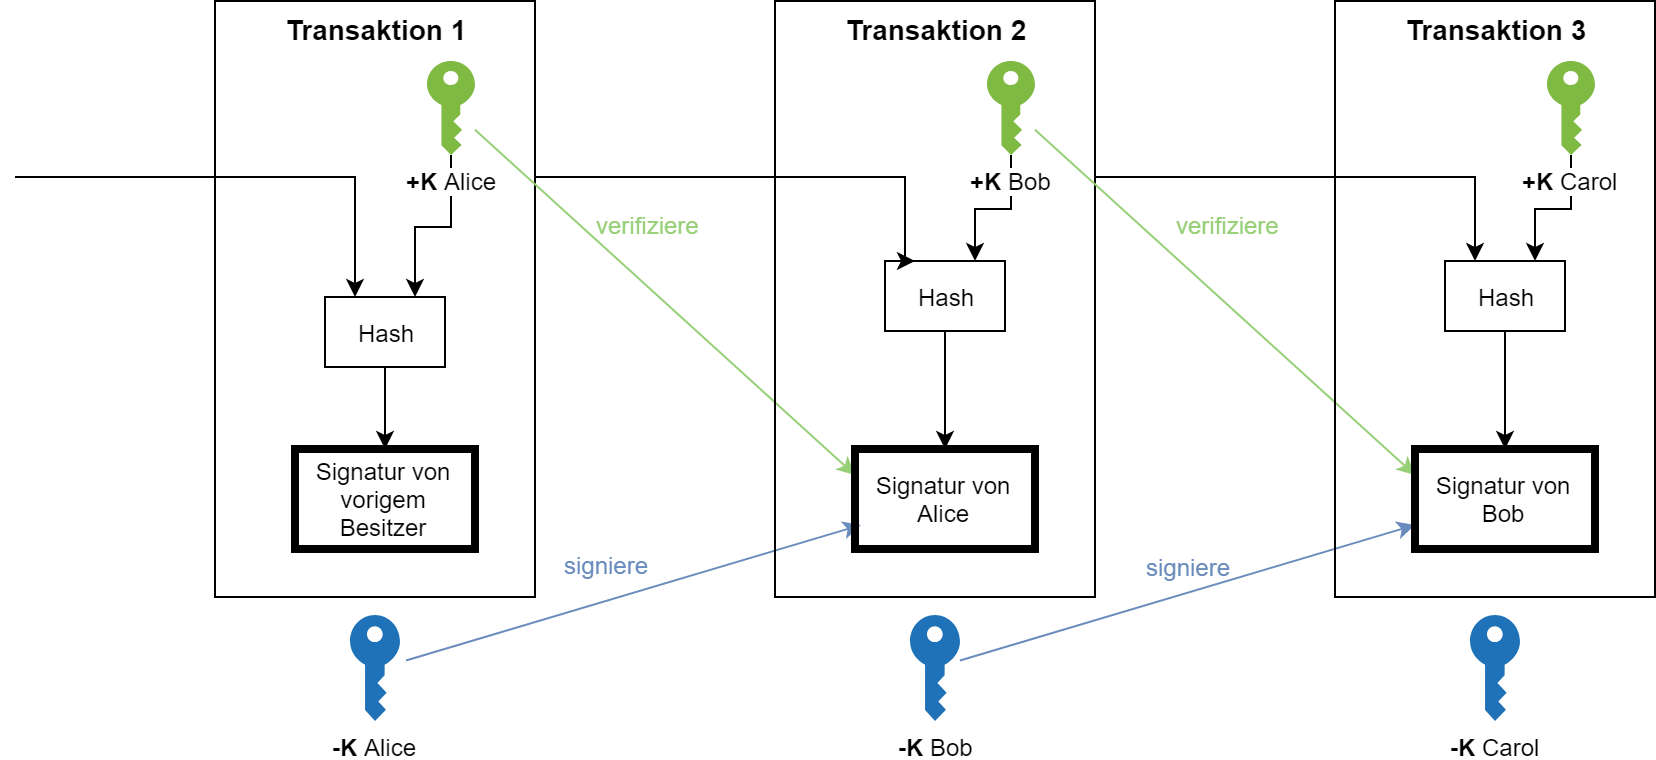
\includegraphics[width=0.9\textwidth]{graphics/transaction.png}
	    	\caption{Kette digitaler Signaturen}
	    	\label{fig:txio}
	    \end{figure}
    
	    Wie in \fref{fig:txio} dargestellt, werden Assets von einem Versender zu einem Empfänger transferiert, in dem der Sender einen Hash der vorigen Transaktion und den öffentlichen Schlüssel des Empfängers mit seinem eigenen privaten Schlüssel digital signiert und diese Hash dann am Ende des Assets anfügt.
	    Transaktionen können zudem mehrere Ein- und Ausgaben haben\cite{Nakamoto2008}.
	    Der Empfänger, sowie alle Teilnehmer des Netzwerkes können den Besitz des Assets über die Kette der digitalen Signaturen zurückverfolgen\cite{Nakamoto2008}.
    
    \begin{figure}[H]
        \missingfigure[figheight=4cm]{Bild mit Transaktion}
    \end{figure}
    
    \subsubsection{Smart Contracts}
    
    \subsubsection{Typen}
        Private, Public - Permissioned, Permissionless
        
        Mit einer Blockchain können auch je nach Anwendungsszenario, außer Kryptowährungen, andere (digital repräsentierte) Waren oder Assets wie Güter im Supply Chain Management\cite{Underwood2016}, Identitäten zur Zugangskontrolle\cite{Kshetri2017} oder Proof of Ownership digitaler Rechte\cite{Wuest2017} gespeichert und gehandelt werden. 
        Unterschiedliche Anwendungen haben auch verschiedene Anforderungen an die Blockchain selbst. 
        Zur Zeit haben sich unterschiedliche Typen einer Blockchain herauskristallisiert, wo.
        
        
        {\sloppy\url{https://blockchainhub.net/blockchains-and-distributed-ledger-technologies-in-general/}}
        \begin{itemize}[noitemsep]
            \item in private/\-permissioned ist \gls{pow} und \gls{pos} nicht nötig
        \end{itemize}
    
    \subsubsection{Sicherheit}
    \label{sec:sota_blockchain_security}
        Byzantine Fault Tolerance
        Consensus Algorithms
    
    \subsubsection{Identity Management}
    \label{sec:sota_blockchain_identitymgmnt}
